\begin{problem}{\#1 (20 points)}
    The following grammar has $\Lambda$-productions, but $\Lambda$ is not in the language generated by this grammar.
    Using the algorithm in chapter 13, find another grammar for the same language that does not have any $\Lambda$-productions.
    \begin{enumerate}[label=\alph*)]
        \item $S \to bZ$\\
        $Z \to ABAB$\\
        $A \to a | \Lambda$\\
        $B \to b | \Lambda$
        \item $S \to aX | bX$\\
        $X \to a | b | \Lambda$\\
    \end{enumerate}
\end{problem}
\begin{solution}
    \begin{enumerate}[label=\alph*)]
        \item $S \to bZ$\\
        $Z \to ABAB | BAB | ABA | BA | AB | A | B$\\
        $A \to a$\\
        $B \to b$
        \item $S \to aX | bX | a | b$\\
        $X \to a | b$
    \end{enumerate}
\end{solution}

\begin{problem}{\#2 (20 points)}
    The following context-free grammar (CFG) has unit productions.
    Using the algorithm presented in chapter 13, find a CFG for the same language that does not have any unit productions.
    \begin{enumerate}[label=\alph*)]
        \item $S \to aXZa | aXa | aZa | aa$\\
        $X \to Y | a$\\
        $Y \to Z | b$\\
        $Z \to bZ | b$
        \item $S \to aX | Yb$\\
        $X \to S$\\
        $Y \to bY | b$
    \end{enumerate}
\end{problem}
\begin{solution}
    \begin{enumerate}[label =\alph*)]
        \item $S \to aXZa | aXa | aZa | aa$\\
        $X \to a | b | bZ$\\
        $Z \to bZ | b$
        \item $S \to aX | Yb$\\
        $X \to aX | Yb$\\
        $Y \to bY | b$
    \end{enumerate}
\end{solution}

\begin{problem}{\#3 (20 points)}
    Convert the grammar you obtained as a result of Question 2 into Chomsky Normal Form (CNF).
\end{problem}
\begin{solution}
    \begin{enumerate}[label=\alph*)]
        \item $S \to R_1R_2 | R_1A | AR_2 | AA $\\
        $X \to a | b | BZ$\\
        $Z \to b | BZ$\\
        $R_1 \to AX$\\
        $R_2 \to ZA$\\
        $A \to a$\\
        $B \to b$
        \item $S \to AX | YB$\\
        $X \to AX | YB$\\
        $Y \to YB | b$\\
        $A \to a$\\
        $B \to b$
    \end{enumerate}
\end{solution}

\begin{problem}{\#4 (20 points)}
    Convert the following CFG into CNF.
    \begin{enumerate}[label=\alph*)]
        \item $S \to aXX$\\
        $X \to aS | bS | a$
        \item $E \to E + E$\\
        $E \to E * E$\\
        $E \to \left( E \right)$\\
        $E \to 7$ 
    \end{enumerate}
\end{problem}
\begin{solution}
    \begin{enumerate}[label=\alph*)]
        \item $S' \to AR_1$\\
        $S \to AR_1$\\
        $X \to AS|BS|a$\\
        $R_1 \to XX$\\
        $A \to a$\\
        $B \to b$
        \item $E' \to R_1E | R_2E | R_3E | 7$\\
        $E \to R_1E | R_2E | R_3) | 7$\\
        $R_1 \to E+$\\
        $R_2 \to E*$\\
        $R_2 \to (E$\\
    \end{enumerate}
\end{solution}

\begin{problem}{\#5 (15 points)}
    Consider the following push down automation (PDA).
    \begin{center}
        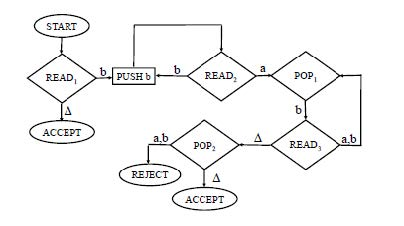
\includegraphics[width=\linewidth]{figures/question5.jpg}
    \end{center}
    \begin{enumerate}[label=\alph*)]
        \item Using a trace table like those in Chapter 14, show what happens to the input tape and stack as each of the following words proceeds through the machine.
        \begin{enumerate}[label=\arabic*)]
            \item $bbbaaa$
            \item $bbbbaa$
        \end{enumerate}
        \item What is the language accepted by this PDA?
        Write English description of the language.
    \end{enumerate}
\end{problem}
\begin{solution}
    \begin{enumerate}[label=\alph*)]
        \item \begin{enumerate}[label=\arabic*)]
            \item \begin{table}[H]
                \centering\begin{tabular}{|c|c|c|}
                    \hline
                    \textbf{STATE} & \textbf{STACK} & \textbf{TAPE} \\
                    \hline
                    START & $\Delta$ & bbbaaa$\Delta$\\
                    \hline
                    $\text{READ}_1$ & $\Delta$ & \sout{b}bbaaa$\Delta$\\
                    \hline
                    PUSH b & b$\Delta$ &\sout{b}bbaaa$\Delta$\\
                    \hline
                    $\text{READ}_2$ & b$\Delta$ & \sout{bb}baaa$\Delta$\\
                    \hline
                    PUSH b & bb$\Delta$ &\sout{bb}baaa$\Delta$\\
                    \hline
                    $\text{READ}_2$ & bb$\Delta$ & \sout{bbb}aaa$\Delta$\\
                    \hline
                    PUSH b & bbb$\Delta$ &\sout{bbb}aaa$\Delta$\\
                    \hline
                    $\text{READ}_2$ & bbb$\Delta$ & \sout{bbba}aa$\Delta$\\
                    \hline
                \end{tabular}
                \quad
                \begin{tabular}{|c|c|c|}
                    \hline
                    \textbf{STATE} & \textbf{STACK} & \textbf{TAPE} \\
                    \hline
                    $\text{POP}_1$ & bb$\Delta$ &\sout{bbba}aa$\Delta$\\
                    \hline
                    $\text{READ}_3$ & bb$\Delta$ & \sout{bbbaa}a$\Delta$\\
                    \hline
                    $\text{POP}_1$ & b$\Delta$ &\sout{bbbaa}a$\Delta$\\
                    \hline
                    $\text{READ}_3$ & b$\Delta$ & \sout{bbbaaa}$\Delta$\\
                    \hline
                    $\text{POP}_1$ & $\Delta$ &\sout{bbbaaa}$\Delta$\\
                    \hline
                    $\text{READ}_3$ & $\Delta$ & \sout{bbbaaa$\Delta$}\\
                    \hline
                    $\text{POP}_2$ & &\sout{bbbaaa$\Delta$}\\
                    \hline
                    ACCEPT & & \sout{bbbaaa$\Delta$}\\
                    \hline
                \end{tabular}
            \end{table}
            \item \begin{table}[H]
                \centering\begin{tabular}{|c|c|c|}
                    \hline
                    \textbf{STATE} & \textbf{STACK} & \textbf{TAPE} \\
                    \hline
                    START & $\Delta$ & bbbbaa$\Delta$\\
                    \hline
                    $\text{READ}_1$ & $\Delta$ & \sout{b}bbbaa$\Delta$\\
                    \hline
                    PUSH b & b$\Delta$ &\sout{b}bbbaa$\Delta$\\
                    \hline
                    $\text{READ}_2$ & b$\Delta$ & \sout{bb}bbaa$\Delta$\\
                    \hline
                    PUSH b & bb$\Delta$ &\sout{bb}bbaa$\Delta$\\
                    \hline
                    $\text{READ}_2$ & bb$\Delta$ & \sout{bbb}baa$\Delta$\\
                    \hline
                    PUSH b & bbb$\Delta$ &\sout{bbb}baa$\Delta$\\
                    \hline
                    $\text{READ}_2$ & bbb$\Delta$ & \sout{bbbb}aa$\Delta$\\
                    \hline
                \end{tabular}
                \quad
                \begin{tabular}{|c|c|c|}
                    \hline
                    \textbf{STATE} & \textbf{STACK} & \textbf{TAPE} \\
                    \hline
                    PUSH b & bbbb$\Delta$ &\sout{bbbb}aa$\Delta$\\
                    \hline
                    $\text{READ}_2$ & bbbb$\Delta$ & \sout{bbbba}a$\Delta$\\
                    \hline
                    $\text{POP}_1$ & bbb$\Delta$ &\sout{bbbba}a$\Delta$\\
                    \hline
                    $\text{READ}_3$ & bbb$\Delta$ & \sout{bbbbaa}$\Delta$\\
                    \hline
                    $\text{POP}_1$ & bb$\Delta$ &\sout{bbbbaa}$\Delta$\\
                    \hline
                    $\text{READ}_3$ & bb$\Delta$ & \sout{bbbbaa$\Delta$}\\
                    \hline
                    $\text{POP}_3$ & b$\Delta$ &\sout{bbbbaa$\Delta$}\\
                    \hline
                    REJECT & b$\Delta$ &\sout{bbbbaa$\Delta$}\\
                    \hline
                \end{tabular}
            \end{table}
        \end{enumerate}
        \item The language accepted by this PDA is any number of $b$'s followed by the same number of $a$'s.
    \end{enumerate}
\end{solution}

\begin{problem}{\#6 (10 points)}
    Convert the following FA into equivalent PDA.
    \begin{center}
        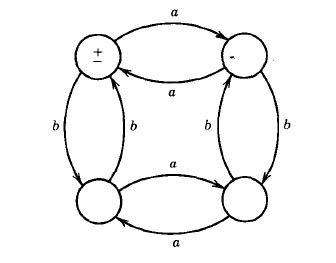
\includegraphics[]{figures/question6.jpg}
    \end{center}
\end{problem}
\begin{solution}
    \begin{center}
        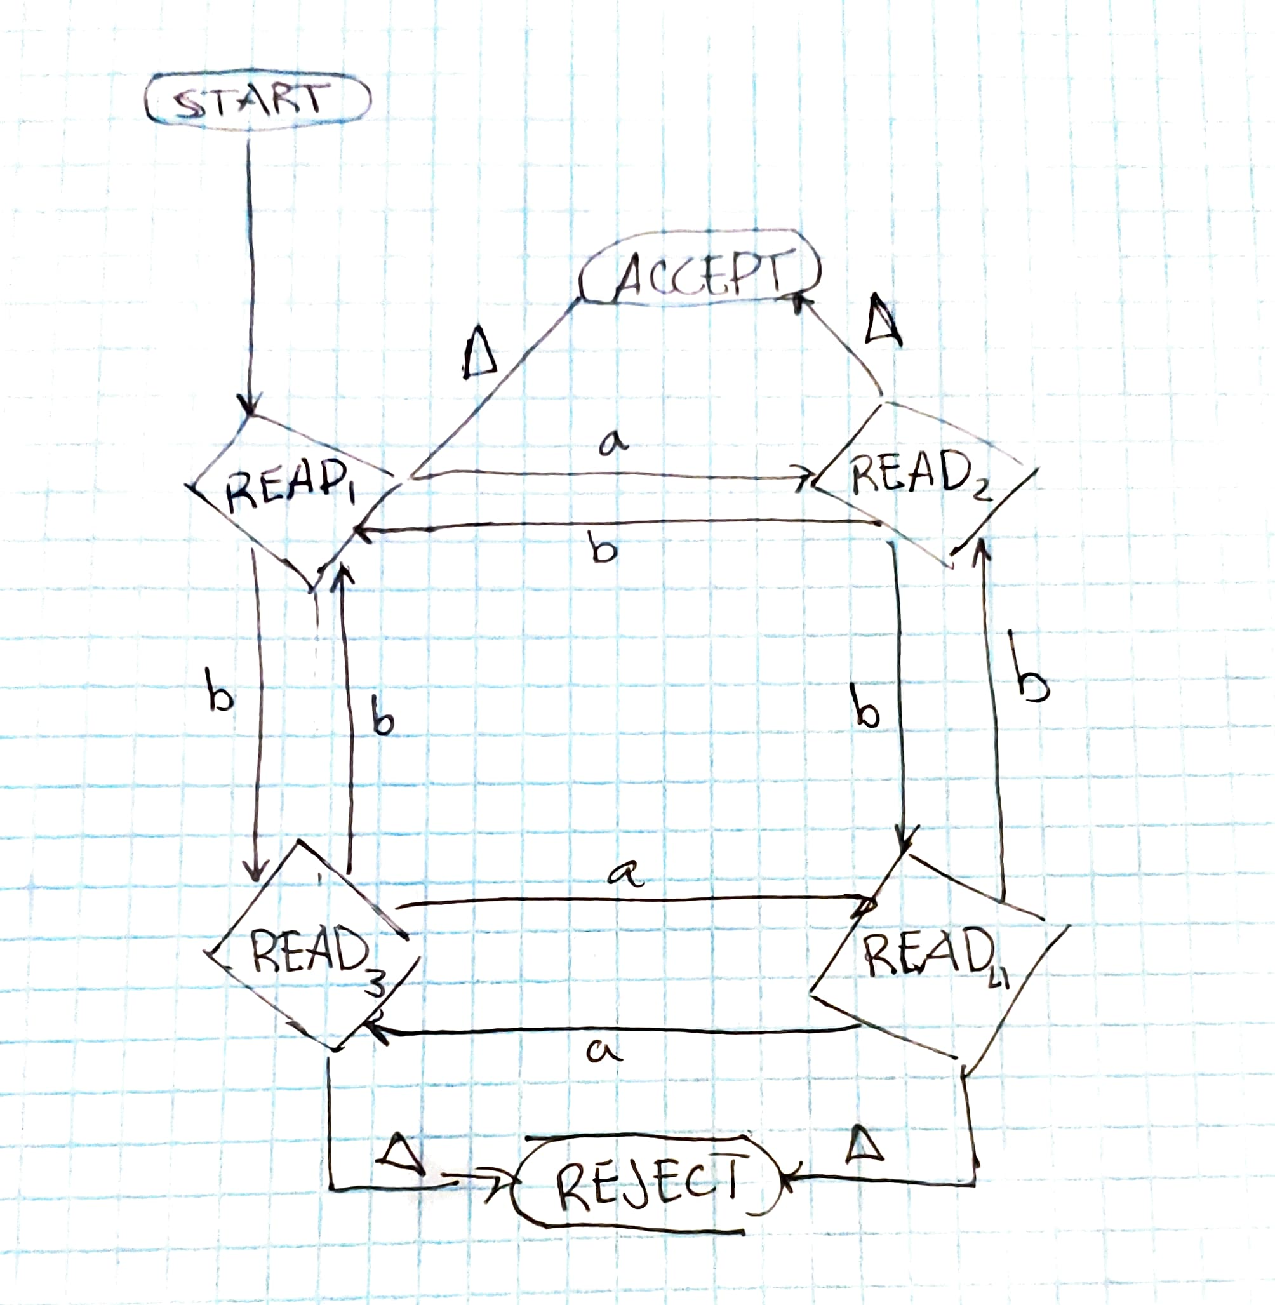
\includegraphics[width=\linewidth]{figures/answer.pdf}
    \end{center}
\end{solution}

\begin{problem}{\#7 (20 points)}
    For a given CFG, construct a PDA that accepts the same language they generate, using the algorithm in chapter 15?
    \\
    Note: Make sure that CFG in proper format to convert it into PDA.
    \begin{enumerate}[label=\alph*)]
        \item $S \to XY$\\
        $X \to aX | bX | a$\\
        $Y \to Ya | Yb | a$
        \item $S \to aS | aSbS | a$
    \end{enumerate}
\end{problem}
\begin{solution}
    \begin{enumerate}[label=\alph*)]
        \item \begin{center}
            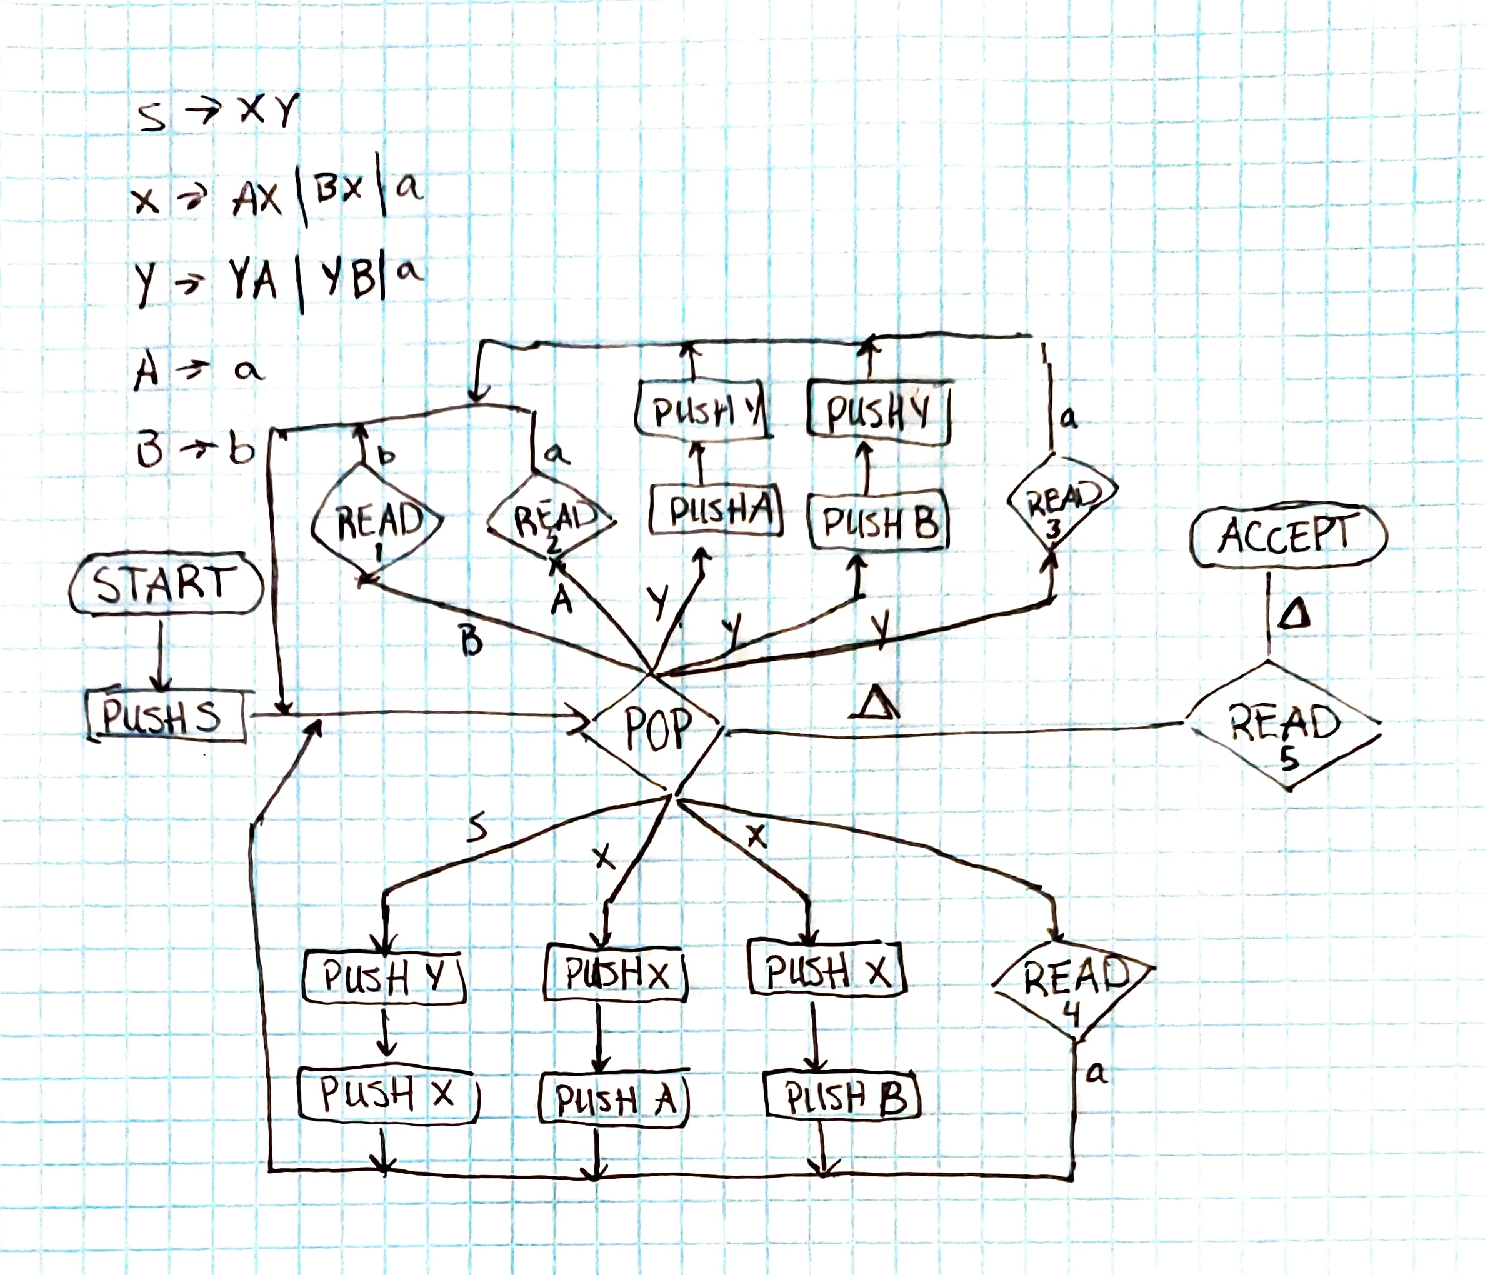
\includegraphics[width=\linewidth]{figures/answer7a.pdf}
        \end{center}
        \item \begin{center}
            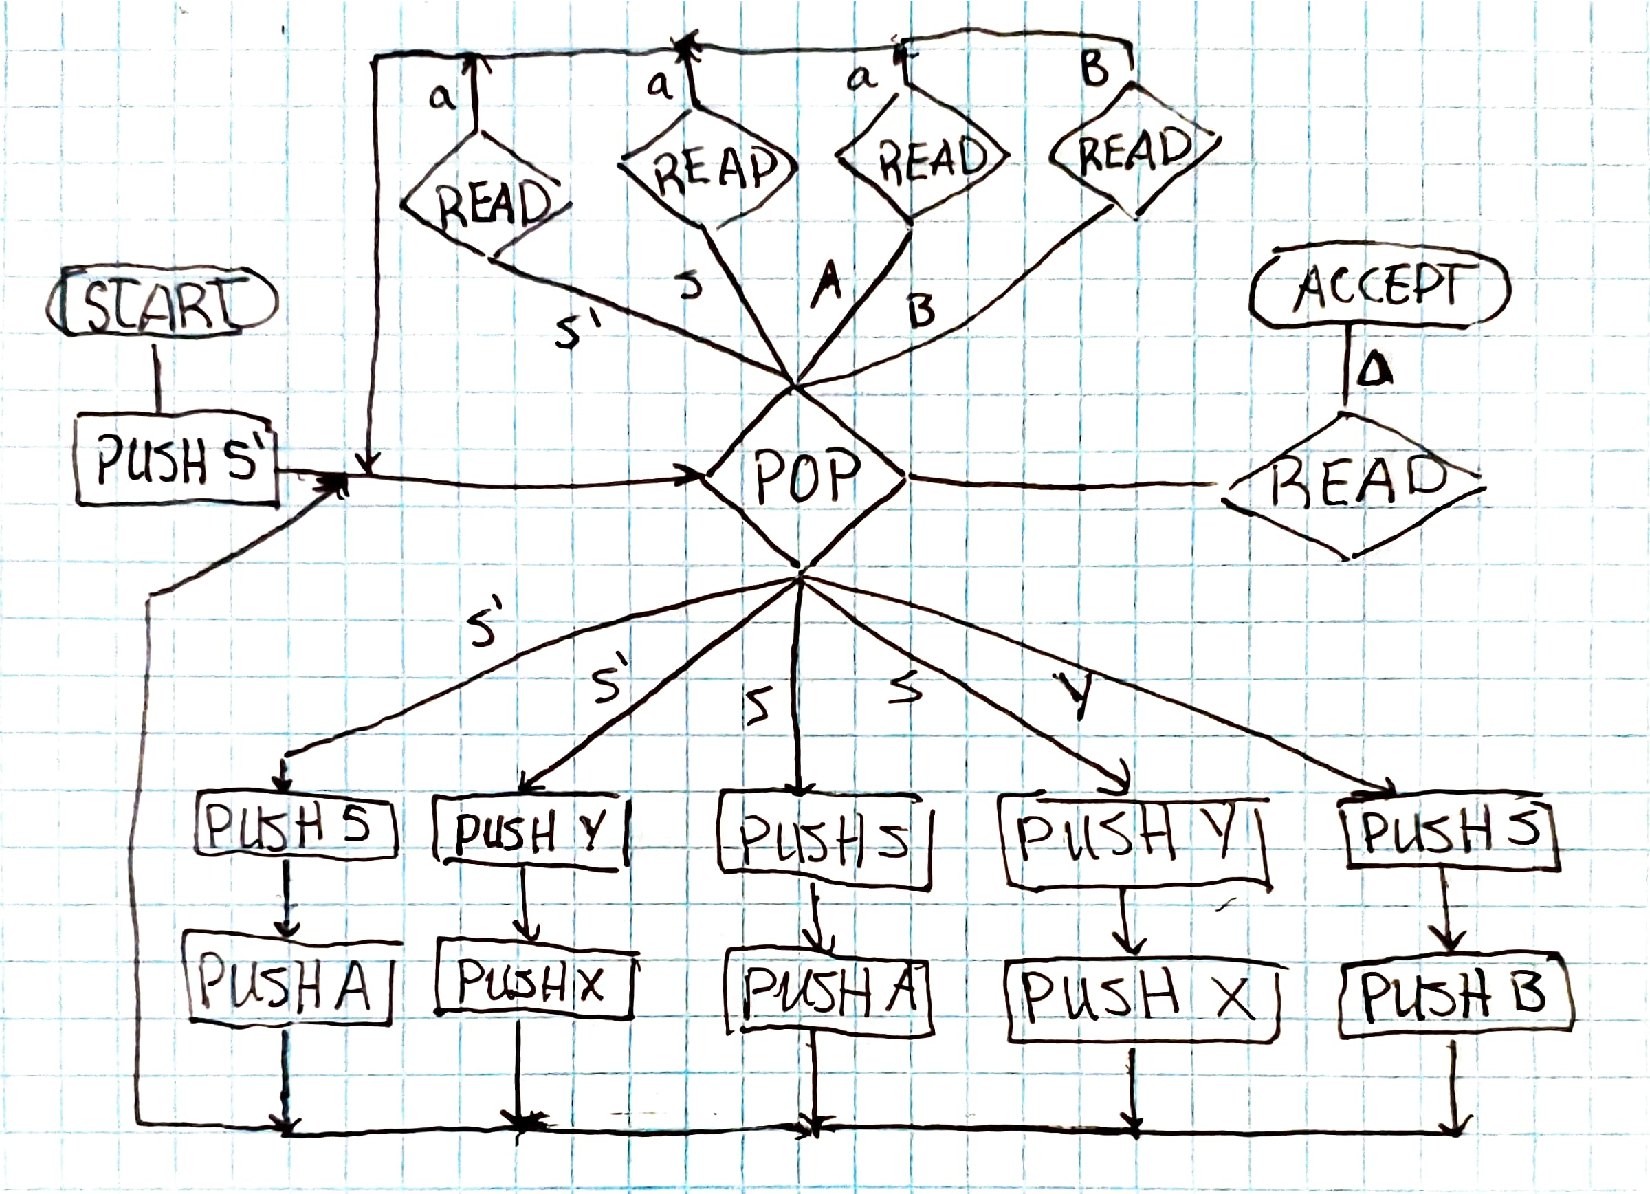
\includegraphics[width=\linewidth]{figures/answer7b.pdf}
        \end{center}
    \end{enumerate}
    
\end{solution}